\documentclass{standalone}
\usepackage{tikz}
\usepackage{ctex,siunitx,ninecolors}
\setCJKmainfont{Noto Serif CJK SC}
\usepackage{tkz-euclide}
\usepackage{amsmath}
\usepackage{wasysym}
\usetikzlibrary{patterns, calc}
\usetikzlibrary{decorations.pathmorphing, decorations.pathreplacing, decorations.shapes,3d}
\begin{document}
\small
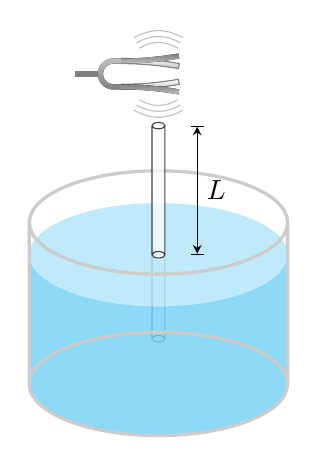
\begin{tikzpicture}[>=stealth,scale=0.82]
  \begin{scope}[rotate=-90,yshift=-0.7cm,xshift=-5.8cm,scale=0.4,
    ]
    \fill[gray](0.1,-0.45)rectangle(-0.1,-1.5);
    \fill[top color=lightgray,bottom color=gray](-0.4,0)arc(180:360:0.4)--++(0,0.3)--++(0.2,0)--++(0,-0.3)arc(0:-180:0.6)--++(0,0.3)--++(0.2,0)--cycle;
    \filldraw[draw=gray,bottom color=lightgray,top color=white](0.6,0.3)arc(0:10:13)--++(190:0.2)arc(10:0:12.8);
    \filldraw[draw=gray,bottom color=lightgray,top color=white](-0.4,0.3)arc(180:170:12.8)--++(170:0.2)arc(170:180:13);
    \fill[bottom color=lightgray,top color=gray](-0.4,0.3)arc(0:10:13)--++(190:0.2)arc(10:0:12.8);
    \fill[bottom color=lightgray,top color=gray](0.6,0.3)arc(180:170:12.8)--++(170:0.2)arc(170:180:13);
    \draw[lightgray](1.0,1.0)to[bend right](1.0,2.5);
    \draw[lightgray](1.2,0.9)to[bend right](1.2,2.6);
    \draw[lightgray](1.4,0.8)to[bend right](1.4,2.7);
    \draw[lightgray](-1.0,1.0)to[bend left](-1.0,2.5);
    \draw[lightgray](-1.2,0.9)to[bend left](-1.2,2.6);
    \draw[lightgray](-1.4,0.8)to[bend left](-1.4,2.7);
  \end{scope}
  \draw[lightgray](-0.1,1.7)--(-0.1,3)(0.1,1.7)--(0.1,3)(0,1.7)ellipse(0.1 and 0.05);
  \fill[cyan!50,opacity=0.5](0,3)ellipse(2.0 and 0.8);
  \fill[cyan!90,opacity=0.5](2.0,1.0)--++(0,2)arc(360:180:2.0 and 0.8)--++(0,-2)arc(180:360:2.0 and 0.8);
  \draw[very thick,lightgray!80](0,1)ellipse(2.0 and 0.8)(0,3.5)ellipse(2.0 and 0.8)(-2,1)--(-2,3.5)(2,1)--(2,3.5);
  \fill[white,opacity=0.7](-0.1,3)--(-0.1,5)arc(180:0:0.1 and 0.05)--(0.1,3)arc(360:180:0.1 and 0.05);
  \draw[darkgray](-0.1,3)--(-0.1,5)(0.1,3)--(0.1,5)(0,3)ellipse(0.1 and 0.05)(0,5)ellipse(0.1 and 0.05);
  \draw[|<->|](0.6,3)--(0.6,5)node[midway,right]{$L$};
\end{tikzpicture}
\end{document}